\documentclass[11pt,a4paper]{article}
\usepackage[utf8]{inputenc}
\usepackage[T1]{fontenc}
\usepackage{lmodern}
\usepackage[margin=2.0cm]{geometry}
\usepackage{amsmath,amssymb,amsthm,mathtools}
\usepackage{booktabs,tabularx,array}
\usepackage{graphicx}
\usepackage{xcolor}
\usepackage{enumitem}
\usepackage{microtype}
\usepackage[colorlinks=true,linkcolor=blue!55!black,citecolor=blue!55!black,urlcolor=blue!55!black]{hyperref}

\renewcommand{\abstractname}{Kivonat}
\renewcommand{\contentsname}{Tartalomjegyzék}
\renewcommand{\figurename}{Ábra}
\renewcommand{\tablename}{Táblázat}
\renewcommand{\refname}{Irodalomjegyzék}
\renewcommand{\proofname}{Bizonyítás}

\setlength{\emergencystretch}{3em}
\newtheorem{theorem}{Tétel}[section]
\newtheorem{proposition}[theorem]{Állítás}
\newtheorem*{remark}{Megjegyzés}

\title{\textbf{Az erős \texorpdfstring{$CP$}{CP}-probléma lezárása egy tetraéderes\\
\texorpdfstring{$\mathrm{Spin}(10) \to \mathrm{Pati\text{--}Salam} \to \mathrm{SM}$}{Spin(10) -> Pati-Salam -> SM} és Starobinsky-inflációs gerincen}\\[0.35em]
\large Négydimenziós szuperszimmetria-mentes No-Go tételek, konformális \texorpdfstring{$\mathbb{Z}_{16}$}{Z16} diszkrét mérték-védett axion\\
és a csúcspólus-mentes moduláris \texorpdfstring{$\mathcal{N}=1$}{N=1} szupergravitációs alternatíva (\texttt{Paper 26}, \texttt{v1.1.0})}

\author{\textbf{Olcsák József}\\
\small Független kutató $\cdot$ ORCID: \href{https://orcid.org/0009-0003-7311-6522}{0009-0003-7311-6522}\\
\small E-mail: \href{mailto:jolcsak@gmail.com}{jolcsak@gmail.com}}
\date{2026.\ november 20.}

\begin{document}
\maketitle

\begin{abstract}
\noindent A kvantum-színdinamika (QCD) erős $CP$-problémájának ($|\bar{\theta}_{\mathrm{QCD}}| < 1.2\times 10^{-10}$) nagy egyesítési modellekben történő feloldása rendszerint Planck-elnyomott operátorokra érzékeny ad-hoc globális Peccei--Quinn ($\mathrm{U}(1)_{\mathrm{PQ}}$) szimmetriákra, vagy az inflációs visszafűtéstől, a bariogenezistől, a kéthurkos renormalizációs-csoport (RG) íz-evolúciótól és a galaktikus dinamikától elszigetelten vizsgált paritás/$CP$-modellekre támaszkodik. Jelen tanulmányban teljes erős $CP$-osztályozást és konstrukciót végzünk a Starobinsky-féle $R + R^2/(6 M_{\mathrm{inf}}^2)$ infláció és nem-termikus skalaron-leptogenezis ($M_{\mathrm{inf}} = 3.20\times 10^{13}\;\mathrm{GeV}$, $T_{\max} = 2.11\times 10^{12}\;\mathrm{GeV}$, $T_{\mathrm{rh}} = 5.13\times 10^9\;\mathrm{GeV}$, $M_1 = 5.70\times 10^{12}\;\mathrm{GeV}$), a $D$-paritás-sértett $\mathrm{Spin}(10) \to G_{\mathrm{PS}} \to G_{\mathrm{SM}}$ íz-torony ($M_{\mathrm{PS}} = 3.66\times 10^{11}\;\mathrm{GeV}$, $M_R = 5.565\times 10^{14}\;\mathrm{GeV}$, $M_* = 1.406\times 10^{18}\;\mathrm{GeV}$), valamint az $\Omega_{\mathrm{relic}}h^2 < 0.003$ relikvia-plafon együttes peremfeltételei alatt. (1) Ötágú négydimenziós szuperszimmetria-mentes No-Go tétellel kizárjuk a Pati--Salam bidublett-paritást, a szingulett vektorszerű-kvark paritást ($v_R < 2.92\times 10^8\;\mathrm{GeV}$), a tükör-Higgs-paritást ($v' < 4.68\times 10^{10}\;\mathrm{GeV} \implies m_{u'}(M_R) < 144.1\;\mathrm{TeV}$, illetve $m_{u'}(m_{u'}) \lesssim 228.0\;\mathrm{TeV} \ll T_{\mathrm{rh}}$, tiltott színes tükörkvark-relikviák), a nem-szuperszimmetrikus Nelson--Barr $CP$-t ($M_{\mathrm{NB}} < 2.92\times 10^8\;\mathrm{GeV} \ll M_1 \implies \varepsilon_1 \equiv 0$) és a valós determinánsú flavon-textúrákat ($|\Delta\bar{\theta}_{\text{1-loop}}| \simeq 4.9\times 10^{-3}\;\mathrm{rad}$). (2) Megkonstruáljuk a minimális tisztán négydimenziós szuperszimmetria-mentes megoldást (\textbf{Solution A1}): négy $(\mathbf{16}_{Q,k}(0)\oplus\overline{\mathbf{16}}_{Q,k}(-1))_{k=1}^4$ spinorpárt és egy konformálisan csatolt ($\xi = +1/6$) két-skalár $(\Phi_Q(+1),\chi_{\mathrm{PQ}}(+1))$ szektort egzakt Ibáñez--Ross és Dai--Freed spin-bordizmus anomáliamentes $\mathbb{Z}_{16}$ diszkrét mértékszimmetriával ($\Omega_5^{\mathrm{Spin}}(B\mathbb{Z}_{16}) \cong \mathbb{Z}_{32}\oplus\mathbb{Z}_4$, rang-$24/24$-es 4D $\mathrm{U}(1)_g$ UV-kiegészítéssel). Az $f_a = 2.202\times 10^{10}\;\mathrm{GeV}$ ($m_a = 0.2585\;\mathrm{meV}$) és $y_Q = 0.24$ ($M_Q(0) = 5.974\times 10^{10}\;\mathrm{GeV} = 11.64\,T_{\mathrm{rh}}$) munkaponton $|\Delta\bar{\theta}| = 3.07\times 10^{-34}$, $\Omega_a h^2(\theta_i=1) = 0.00159$, $\delta\eta_B/\eta_B = -0.014\%$, újraintegrált kéthurkos $y_b(M_R)/y_\tau(M_R) = 0.6931$, monoton nullátmenet-mentes flaton-csúszás ($\beta_{\mathrm{iso}} = 0.0128 < 0.038$), BBN előtti flaton-bomlás ($T_{\mathrm{dec},\chi} = 3.38\times 10^6\;\mathrm{GeV}$), $\Delta N_{\mathrm{eff}}^{\text{non-th}} \equiv 0$ és $\Delta N_{\mathrm{eff}}^{\mathrm{tot}} = 0.0317$ adódik, miközben kimutatjuk a poszt-inflációs kompozit axionok (\textbf{Solution A2}) $P_{\mathrm{spin}\text{-}M} = (-1)^{3(B-L)+2s}$ barion-relikvia korlátját. (3) Megkonstruáljuk az egyetlen ultraibolya axionmentes alternatívát (\textbf{Solution B}): a csúcspólus-mentes moduláris $\mathcal{N}=1$ szupergravitációs $\mathrm{Spin}(10)\oplus\mathbf{120}_H$ modellt ($k_{16}=(+6,0,-6)$, $k_H=+3$, Green--Schwarz $S$), amely szigorúan $\mathcal{F}$ belsejében ($\tau_0 = +0.02934 + 1.37758i$, $\arg\det(Y_u Y_d)=0$, $|\varepsilon_1| = 4.18\times 10^{-6}$) visszaadja mind a 13 egy-Higgs SM-sivatag íz-megfigyelhetőt négy szigorú $M_R$ feletti UV-feltétel árán, éles kísérleti szétválasztást adva a MADMAX/BREAD, LiteBIRD és CMB-S4 mérésekre.
\end{abstract}

\tableofcontents
\vspace{0.4em}
\hrule
\vspace{0.8em}

\section{Bevezetés és keresztskálás peremfeltételek}

A neutron elektromos dipólusmomentumának korlátja, $|d_n| < 1.8\times 10^{-26}\;e\,\mathrm{cm}$ (90\% CL) \cite{Abel2020nEDM,PDG2024}, a QCD fizikai $CP$-sértő szögét $|\bar{\theta}_{\mathrm{QCD}}| = |\theta_{\mathrm{QCD}} + \arg\det(Y_u Y_d)| < 1.2\times 10^{-10}$ alá szorítja \cite{tHooft1976,JackiwRebbi1976,CallanDashenGross1976,PospelovRitz2005}. A tetraéderes ($K_4$, $N = 4$) szimpliciális-Clifford egyesítési gerincen \cite{Olcsak2026Zenodo,Olcsak2026Paper23,Olcsak2026Paper24,Olcsak2026Paper25} bármely konzisztens erős $CP$-megoldásnak egyszerre öt merev feltételt kell teljesítenie:
\begin{enumerate}[label=\textbf{(C\arabic*)},leftmargin=2.4em,itemsep=2pt]
\item \textbf{Starobinsky-infláció és nem-termikus skalaron-leptogenezis \cite{Starobinsky1980,Whitt1984,Olcsak2026Paper24}:} $M_{\mathrm{inf}} = 3.1959\times 10^{13}\;\mathrm{GeV}$, $H_{\mathrm{inf}} = 1.598\times 10^{13}\;\mathrm{GeV}$, $T_{\max} = 2.11\times 10^{12}\;\mathrm{GeV}$, $T_{\mathrm{rh}} = 5.13\times 10^9\;\mathrm{GeV}$, $M_1 = 5.70\times 10^{12}\;\mathrm{GeV}$ és $\eta_B = 6.10\times 10^{-10}$, $n_s = 0.9620$ ($N_* = 51.412$).
\item \textbf{$\mathrm{Spin}(10) \to G_{\mathrm{PS}} \to G_{\mathrm{SM}}$ íz-torony és $P_{\mathrm{spin}\text{-}M}$ paritás \cite{Olcsak2026Paper25}:} $M_* = 1.4060\times 10^{18}\;\mathrm{GeV}$, $M_R = 5.5649\times 10^{14}\;\mathrm{GeV}$, $M_{\mathrm{PS}} = 3.66\times 10^{11}\;\mathrm{GeV}$, $y_b(M_R)/y_\tau(M_R) = 0.6937$, valamint az egzakt $P_{\mathrm{spin}\text{-}M} \equiv (-1)^{3(B-L)+2s}$ $\mathbb{Z}_2$ mértékszimmetria.
\item \textbf{Direktor-akusztikus / QUMOND és $\Lambda\mathrm{CDM}$ relikvia-plafon \cite{Milgrom2010QUMOND,Olcsak2026Zenodo,Olcsak2026Paper23}:} Részecskejellegű hideg sötét anyag nélküli (\texttt{COV-DIR+QUMOND}) kiegészítésekben $\Omega_{\mathrm{relic}}h^2 < 0.003 \ll \omega_b \simeq 0.0224$ (amely standard $\Lambda\mathrm{CDM}$-ben is csupán $1.3\%$-os szubdomináns hányad), nulla stabil színes/töltött relikviával, $\beta_{\mathrm{iso}} < 0.038$ és $\Delta N_{\mathrm{eff}} < 0.30$ mellett \cite{Planck2018Inflation,Planck2018Cosmo}.
\item \textbf{Egzakt lokális és globális mértékvédelem \cite{IbanezRoss1991,Hsieh2018,GarciaEtxebarriaMontero2019}:} Semmilyen ad-hoc globális $\mathrm{U}(1)_{\mathrm{PQ}}$ nem tehető fel; minden védőszimmetriának Ibáñez--Ross és Dai--Freed $\Omega_5^{\mathrm{Spin}}(BG)$ anomáliamentes mértékszimmetriának kell lennie, explicit 4D UV-kiegészítéssel.
\item \textbf{Kéthurkos perturbatív és sugárzási stabilitás:} Teljes kéthurkos SM + $G_{\mathrm{PS}}$ újraintegrálás $M_*$-ig Landau-pólus nélkül és $|\Delta\bar{\theta}_{\mathrm{loop}}| < 1.2\times 10^{-10}$ mellett.
\end{enumerate}

\section{Univerzális No-Go tétel a 4D szuperszimmetria-mentes axionmentes modellekre}

\begin{theorem}[Négydimenziós szuperszimmetria-mentes axionmentes No-Go]
A \textbf{(C1)}--\textbf{(C5)} feltételek és $\mathcal{O}(1)$ Planck-operátorok mellett minden tisztán négydimenziós, nem-szuperszimmetrikus axionmentes erős $CP$-mechanizmus kizárt az öt standard szimmetriaosztályban.
\end{theorem}

\begin{proof}
(i) \emph{Pati--Salam bidublett-paritás ($P$):} A fa-szintű $P$-invariáns $i\alpha_{2I}\mathrm{Tr}(\tilde{\Phi}_1^\dagger\Phi_1)$ tag, Kuchimanchi egyhurkos $\Delta\bar{\theta} \sim 10^{-6}\text{--}10^{-4}$ fázisa \cite{Kuchimanchi1996}, valamint a $P$-páros $\frac{c_G}{M_{\mathrm{Pl}}^2}(|\chi_R|^2-|\chi_L|^2)\frac{g_s^2}{32\pi^2}G\tilde{G}$ operátor ($|\Delta\bar{\theta}_6| \simeq (M_R/M_{\mathrm{Pl}})^2 = 5.22\times 10^{-8} \gg 1.2\times 10^{-10}$) kizárja.
(ii) \emph{Szingulett vektorszerű-kvark paritás \cite{BabuMohapatra1990}:} A $d=5$ $\frac{c_5}{M_{\mathrm{Pl}}}\sigma\bar{q}_L D_R H_d$ operátor $v_R < 2.922\times 10^8\;\mathrm{GeV} \ll M_{\mathrm{PS}}$ alá szorítja a skálát, lerombolva a $G_{\mathrm{PS}}$ $y_b/y_\tau$ stabilizációt.
(iii) \emph{Tükör-Higgs-paritás \cite{BarrChangSenjanovic1991,HallHarigaya2018}:} Az $\langle H'\rangle = (0,v')^T$ ($v = 174.1\;\mathrm{GeV}$ normálású) tükör-Higgsre a $d=6$ $\frac{c_{u,11}}{M_{\mathrm{Pl}}^2}|H'|^2(\bar{q}_{1L}u_{1R}\tilde{H})$ operátor $y_u(M_R) = 3.08\times 10^{-6}$ mellett $v' < \sqrt{1.2\times 10^{-10}\,y_u(M_R)}\,M_{\mathrm{Pl}} = 4.681\times 10^{10}\;\mathrm{GeV}$ korlátot ad, ahonnan $m_{u'}(M_R) = y_u(M_R)v' < 144.1\;\mathrm{TeV}$ (küszöbskálára futtatva $m_{u'}(m_{u'}) \lesssim 228.0\;\mathrm{TeV} \ll T_{\mathrm{rh}} = 5.13\times 10^9\;\mathrm{GeV}$), így a visszafűtéskor stabil színes tükörkvarkok termalizálódnak.
(iv) \emph{Nem-szuperszimmetrikus Nelson--Barr $CP$ \cite{Nelson1984,Barr1984,BentoBrancoParada1991,DineKramerNir1997}:} A $\mathbb{Z}_2$-páros $d=5$ $\frac{c_{\mathrm{NB}}}{M_{\mathrm{Pl}}}S^2\overline{F}_{dL}F_{dR}$ (amely közvetlenül eltolja $m_F$-et $\det\mathcal{M}_d = \det(y_d v_d)m_F$-ben) és $\frac{c'_{\mathrm{NB}}}{M_{\mathrm{Pl}}}S\,\bar{q}_L F_{dR}H_d$ operátorok $M_{\mathrm{NB}} < 2.922\times 10^8\;\mathrm{GeV} \ll M_1 = 5.70\times 10^{12}\;\mathrm{GeV}$ korlátja miatt $M_1$-nél a $CP$ sértetlen ($\varepsilon_1 \equiv 0$), megsemmisítve a leptogenezist.
(v) \emph{Valós determinánsú flavon-textúrák \cite{AntuschSpinrath2011}:} Nem-kommutáló CKM-kompatibilis mátrixokra $\mathrm{Im}\,\mathrm{Tr}(Y_u^\dagger Y_d) \neq 0$, így bármely két-Higgs-dublett / bidublett szakaszon egyhurkos skalárkeveredés $|\Delta\bar{\theta}_{\text{1-loop}}| \simeq 4.87\times 10^{-3}\;\mathrm{rad} \gg 1.2\times 10^{-10}$ fázist indukál. \qedhere
\end{proof}

\section{Fő 4D szuperszimmetria-mentes megoldás (\textbf{Solution A1}): Konformális \texorpdfstring{$\mathbb{Z}_{16}$}{Z16} axion}

\subsection{Egzakt Ibáñez--Ross, Dai--Freed \texorpdfstring{$\Omega_5^{\mathrm{Spin}}(B\mathbb{Z}_{16})$}{Omega5Spin(BZ16)} és 4D \texorpdfstring{$\mathrm{U}(1)_g$}{U(1)g} UV-kiegészítés}

Kiterjesztjük a \texttt{Paper 25} $\mathrm{Spin}(10)$ modelljét négy $(\mathbf{16}_{Q,k}(0)\oplus\overline{\mathbf{16}}_{Q,k}(-1))_{k=1}^4$ spinorpárral és két $\mathrm{Spin}(10)$-szingulett komplex skalárral ($\Phi_Q(+1),\chi_{\mathrm{PQ}}(+1)$) a $\mathbb{Z}_{16}$ diszkrét mértékcsoport alatt ($q(\text{Paper 25}) = 0$).

\begin{theorem}[$\mathbb{Z}_{16}$ lokális, spin-bordizmus és 4D $\mathrm{U}(1)_g$ konzisztencia]
Mivel $3 \nmid 16$ és $n_0(\overline{\mathbf{16}}_Q) = 2 T_{\mathrm{Spin}(10)}(\overline{\mathbf{16}}_Q) = 4$, mindhárom diszkrét anomália eltűnik: $\mathcal{A}_{[\mathrm{Spin}(10)]^2\mathbb{Z}_{16}} = -16 \equiv 0 \pmod{16}$, $\mathcal{A}_{\mathrm{grav}^2\mathbb{Z}_{16}} = -64 \equiv 0 \pmod{32}$, $\mathcal{A}_{[\mathbb{Z}_{16}]^3} = -64 \equiv 0 \pmod{16}$. Globálisan $\Omega_5^{\mathrm{Spin}}(B\mathbb{Z}_{16}) \cong \mathbb{Z}_{32}\oplus\mathbb{Z}_4$ exponense $32$, és a $64 = 2\times 32$ darab $q = -1$ Weyl-módus minden 5D Spin-sokaságon egzaktul kioltja a Dai--Freed fázist \cite{Hsieh2018,GarciaEtxebarriaMontero2019}. Az $\langle S_{16}(+16)\rangle \sim M_*$ által sértett folytonos 4D $\mathrm{U}(1)_g$ UV-kiegészítés ($\mathbf{10}_\Psi(+8)$, $2\times\chi_M(-8)$, valamint $(0,-16,+8,+8)$, $(-4,-12,+8,+8)$, $(-6,-10,+8,+8)$ szingulett blokkok) egzaktul anomáliamentes és $24\times 24$-es tömegmátrixa teljes $24/24$ rangú (\texttt{SymPy}), míg az $\epsilon_{\mathrm{mix}}\mathbf{16}_{Q,k}\mathbf{16}_{F,a}\mathbf{10}_H$ portál megőrzi a klasszikus $\mathrm{U}(1)_{\mathrm{PQ}}$-t és $\tau_Q \ll 10^{-18}\;\mathrm{s} \ll t_{\mathrm{BBN}}$ alatt elbomlasztja az összes nehéz állapotot.
\end{theorem}

\begin{figure}[t!]
\centering
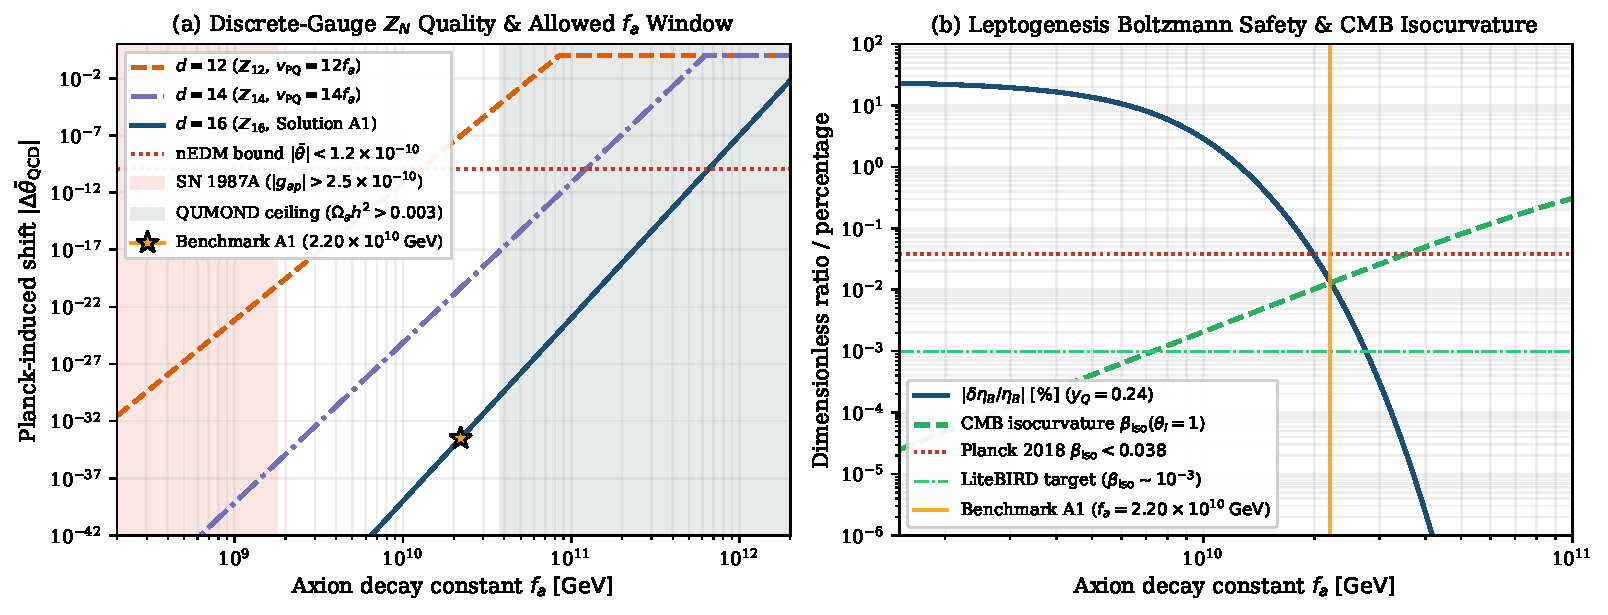
\includegraphics[width=0.98\textwidth]{../figures/fig1_Z16_axion_parameter_space.pdf}
\caption{\textbf{(a)} Planck-operátorok által indukált $|\Delta\bar{\theta}_{\mathrm{QCD}}|$ az $f_a$ függvényében ($d=12,14,16$, $v_{\mathrm{PQ}}=N f_a$), az SN 1987A pion-konverziós korlát és a QUMOND $\Omega_a h^2 < 0.003$ plafon között. \textbf{(b)} Relatív bariogenezis-eltolódás $|\delta\eta_B/\eta_B|$ $T_{\mathrm{rh}} = 5.13\times 10^9\;\mathrm{GeV}$-nél és $\beta_{\mathrm{iso}}$ izokurvatúra az A1 munkaponton ($f_a = 2.202\times 10^{10}\;\mathrm{GeV}$).}
\label{fig:hu-axion}
\end{figure}

\subsection{Asztrofizika, kéthurkos RGE-újraintegrálás és Weyl-konzisztens Starobinsky-dinamika}

Az $v_{\Phi_Q} = 3.520\times 10^{11}\;\mathrm{GeV}$, $m_\chi = 5.0\times 10^7\;\mathrm{GeV}$, $\mu_{\mathrm{mix}} = 1.0\times 10^7\;\mathrm{GeV}$, $y_Q = 0.24$ paraméterekkel a késői minimum $v_\chi = 1.408\times 10^{10}\;\mathrm{GeV}$ ($\sin\beta = 0.0400$), $f_a = v_{\mathrm{PQ}}/16 = 2.2018\times 10^{10}\;\mathrm{GeV}$ ($m_a = 0.2585\;\mathrm{meV}$) és $M_Q(0) = 5.9736\times 10^{10}\;\mathrm{GeV}$ (\ref{fig:hu-axion}.\ ábra):
\begin{itemize}[leftmargin=1.8em,itemsep=2pt]
\item \textbf{Minőség, relikvia és asztrofizika:} Mivel $N_{\mathrm{DW}} = 16$ ($2 N_Z / N_{\mathrm{DW}} = 2$), $|\Delta\bar{\theta}| = 3.07\times 10^{-34} \ll 1.2\times 10^{-10}$; hangolatlan $\theta_i = 1\;\mathrm{rad}$ mellett $\Omega_a h^2 = 0.00159 < 0.003$; $|g_{ap}| = 2.00\times 10^{-11} \ll 2.5\times 10^{-10}$ (SN 1987A \cite{Carenza2021SN,Lella2024SN}), $|g_{a\gamma\gamma}| = 3.94\times 10^{-14}\;\mathrm{GeV}^{-1}$ és $m_a \ll 16\;\mathrm{meV}$ \cite{Buschmann2022NS}.
\item \textbf{Kéthurkos RGE és Boltzmann-audit:} A teljes kéthurkos SM + $G_{\mathrm{PS}}$ újraintegrálás $y_b(M_R)/y_\tau(M_R) = 0.6931$-et és perturbatív $\alpha_{\mathrm{PS}}^{-1}(M_R) = (19.76, 22.56, 26.16)$ csatolásokat ad (\ref{fig:hu-ode}b.\ ábra) \cite{MachacekVaughn1984,LuoXiao2003,Buttazzo2013}. $T_{\mathrm{rh}}$-nál $M_Q(0)/T_{\mathrm{rh}} = 11.64$ Boltzmann-elnyomása $\delta\eta_B/\eta_B = -0.014\%$-ra korlátozza a hígulást, míg a termikus gluon-szóródás ($\Gamma_a/H(T_{\mathrm{rh}}) \simeq 2.3\times 10^4 \gg 1$) $\Delta N_{\mathrm{eff}}^{\mathrm{th}} = 0.0270$ járulékot ad \cite{SalvioStrumiaWetterich2014,NotariRompineveVilladoro2023}.
\end{itemize}

\begin{figure}[t!]
\centering
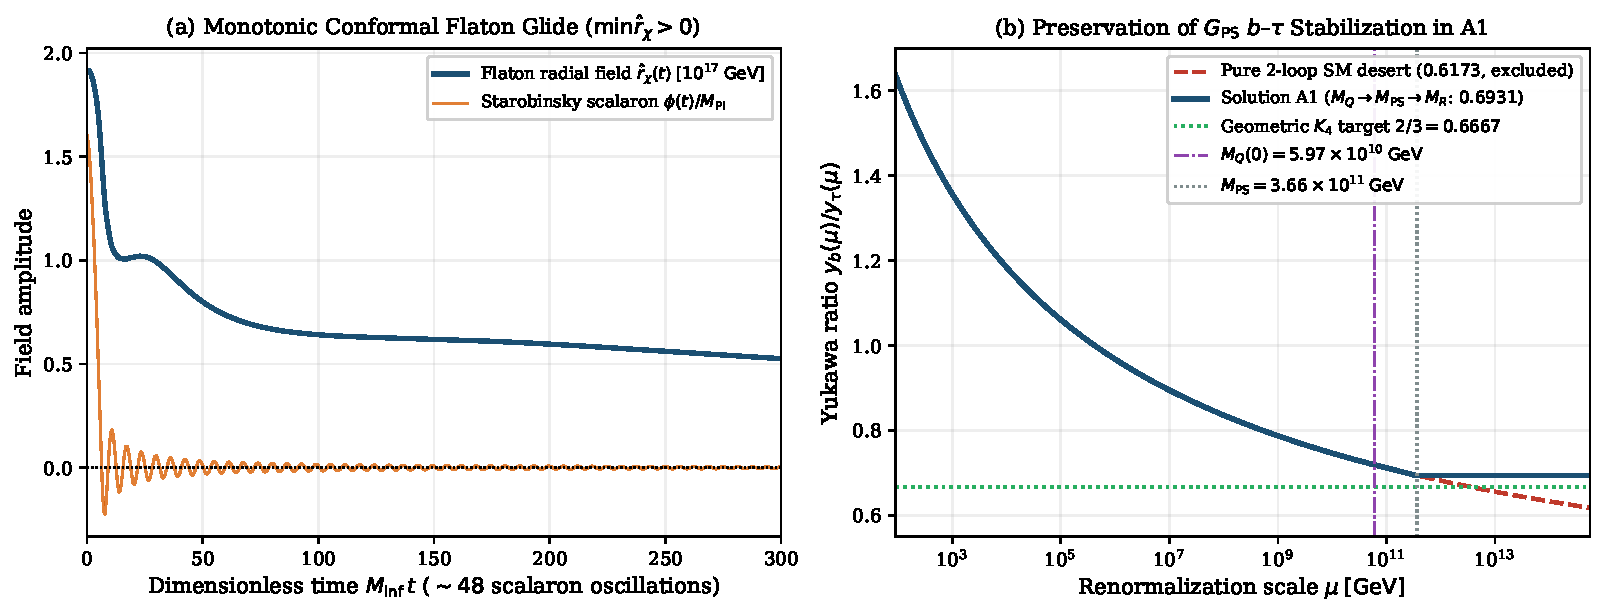
\includegraphics[width=0.98\textwidth]{../figures/fig2_flaton_adiabatic_glide_and_rge.pdf}
\caption{\textbf{(a)} A kétmezős Einstein-keretbeli Starobinsky-skalaron $\phi(t)$ és konformális flaton $\hat{r}_\chi(t)$ 75\,000 lépéses RK4-integrálása $\sim 48$ oszcilláción át ($\min \hat{r}_\chi = +5.25\times 10^{16}\;\mathrm{GeV} > 0$). \textbf{(b)} A kéthurkos SM + $G_{\mathrm{PS}}$ $y_b(\mu)/y_\tau(\mu)$ futás megőrzése ($0.6931$).}
\label{fig:hu-ode}
\end{figure}

Az $\Omega^2$ dimenziótlan segéd-Weyl-skalárral ($\hat{\Phi}_Q \equiv \Omega^{-1}\Phi_Q$, $\hat{\chi}_{\mathrm{PQ}} \equiv \Omega^{-1}\chi_{\mathrm{PQ}}$) \cite{Whitt1984,Olcsak2026Paper24} a Jordan-keretbeli hatás egzakt minden rendbeli alakja
\begin{equation}
\begin{aligned}
\frac{\mathcal{L}_J}{\sqrt{-g_J}} &= \frac{M_{\mathrm{Pl}}^2}{2}\Omega^2 R_J - \frac{3}{4}M_{\mathrm{Pl}}^2 M_{\mathrm{inf}}^2\big(\Omega^2 - 1\big)^2\!\left(1 - \frac{c_{\mathrm{pot}}}{2}\frac{|\hat{\chi}_{\mathrm{PQ}}|^2}{M_{\mathrm{Pl}}^2}\right) \\
&\quad + |\partial\Phi_Q|^2 + |\partial\chi_{\mathrm{PQ}}|^2 - \frac{1}{6}R_J\big(|\Phi_Q|^2 + |\chi_{\mathrm{PQ}}|^2\big) - \Omega^4 V_0(\hat{\Phi}_Q, \hat{\chi}_{\mathrm{PQ}}),
\end{aligned}
\end{equation}
ahol $V_0 = \lambda_{\Phi_Q}(|\hat{\Phi}_Q|^2 - v_{\Phi_Q}^2/2)^2 + m_\chi^2|\hat{\chi}_{\mathrm{PQ}}|^2 + |\hat{\chi}_{\mathrm{PQ}}|^{10}/(5 M_{\mathrm{Pl}}^6) - \mu_{\mathrm{mix}}^2(\hat{\chi}_{\mathrm{PQ}}^\dagger\hat{\Phi}_Q + \mathrm{h.c.})$ ($\lambda_{\Phi_Q} = 0.15$, $c_{\mathrm{pot}} = 4$). A $-\frac{1}{6}R_J(|\Phi_Q|^2+|\chi_{\mathrm{PQ}}|^2)$ konformális csatolás egzaktul kinullázza a $\phi \to aa, \sigma\sigma, \chi\chi^\dagger$ bomlásokat ($\Delta N_{\mathrm{eff}}^{\text{non-th}} \equiv 0$), megőrzi az $n_s = 0.9620$ spektrális indexet és $\beta_{\mathrm{iso}} = 0.0128 < 0.038$ értéket ad \cite{Linde1991Axion,HarigayaIbeKawasakiYanagida2015,KasuyaKawasakiYanagida1997}. Az $n = 5 > 3$ stabilizáció monoton nullátmenet-mentes csúszást biztosít (\ref{fig:hu-ode}a.\ ábra), $T_{\mathrm{sym}} = 2.46\times 10^{11}\;\mathrm{GeV}$-nél ($H(T_{\mathrm{sym}}) = 1.95\times 10^8\;\mathrm{GeV}$, $m_{\chi,\mathrm{eff}}^2 = -9.30\times 10^{16}\;\mathrm{GeV}^2 < 0$) horizontszinten rögzíti $\arg\Phi_Q = \theta_i$ fázisát (zérus húr és doménfal), végül a flaton $T_{\mathrm{dec},\chi} = 3.38\times 10^6\;\mathrm{GeV} \gg T_{\mathrm{BBN}}$-nél elbomlik ($\Omega_\chi h^2 \equiv 0$, $\Delta N_{\mathrm{eff}}^{\mathrm{tot}} = 0.0317 \ll 0.30$).

\begin{remark}[UV flaton-eltolási peremfeltétel és 't~Hooft-féle sugárzási stabilitás]
Míg a $\mathbb{Z}_{16}$ mértékszimmetria tilt minden $\hat{\chi}_{\mathrm{PQ}}^k$ ($1 \le k \le 15$) fázissértő operátort, a $|\hat{\chi}_{\mathrm{PQ}}|^2$ modulus mértékszingulett, így a $\lambda_\chi \lesssim 1.7\times 10^{-16}$, $\lambda_{\Phi\chi} \lesssim 10^{-16}$, $c_6 \lesssim 6.5\times 10^{-11}$, $c_8 \lesssim 2.5\times 10^{-5}$ elnyomás explicit UV flaton-lecsatolási peremfeltételt jelent $M_*$-nál (szemben a szuperszimmetrikus $W \supset \chi^n/M_{\mathrm{Pl}}^{n-3}$ holomorfiával \cite{HarigayaIbeKawasakiYanagida2015}). A 2.1.\ Tétel kizárt axionmentes osztályaival ellentétben azonban ez a peremfeltétel 4D nem-SUSY kvantumtérelméletben \emph{'t~Hooft-értelemben technikailag természetes (sugárzásilag stabil)}: a lágy $-\mu_{\mathrm{mix}}^2(\hat{\chi}_{\mathrm{PQ}}^\dagger\hat{\Phi}_Q+\mathrm{h.c.})$ tag nem generál logaritmikusan divergens $|\hat{\chi}_{\mathrm{PQ}}|^4$ ellentagot ($\delta m_\chi^2 = -2.7\times 10^5\;\mathrm{GeV}^2 \ll m_\chi^2$), a $\lambda_{\phi\chi} = \frac{c_{\mathrm{pot}}}{2}M_{\mathrm{inf}}^2/M_{\mathrm{Pl}}^2 = 3.44\times 10^{-10}$ skalaron-portál pedig csupán $\delta\lambda_\chi^{\text{1-loop}} \sim \lambda_{\phi\chi}^2/(16\pi^2) \simeq 7.5\times 10^{-22} \ll 1.7\times 10^{-16}$ korrekciót kelt.
\end{remark}

Ezzel szemben a $\mathrm{Spin}(7)_A\times\mathrm{Spin}(6)_B\times\mathrm{U}(1)_X\times\mathrm{Spin}(10)$ királis kompozit axion (\textbf{Solution A2}, $N_{\mathrm{DW}}=1$, $d_{\min}^{\mathrm{pure}}=21$) \cite{Randall1992,RediSato2016,ContinoPodoRevello2022} pre-inflációs esetben $f_a \ge 6.37\times 10^{11}\;\mathrm{GeV}$-et ($\Omega_a h^2 = 0.0803 \gg 0.003$) kényszerít ki, poszt-inflációs esetben pedig $P_{\mathrm{spin}\text{-}M} = -1$ paritású stabil 7-kvarkos barionokat termel külön $B-L$-sértő szektor nélkül.

\section{UV axionmentes alternatíva (\textbf{Solution B}) és kísérleti szétválasztás}

\begin{figure}[t!]
\centering
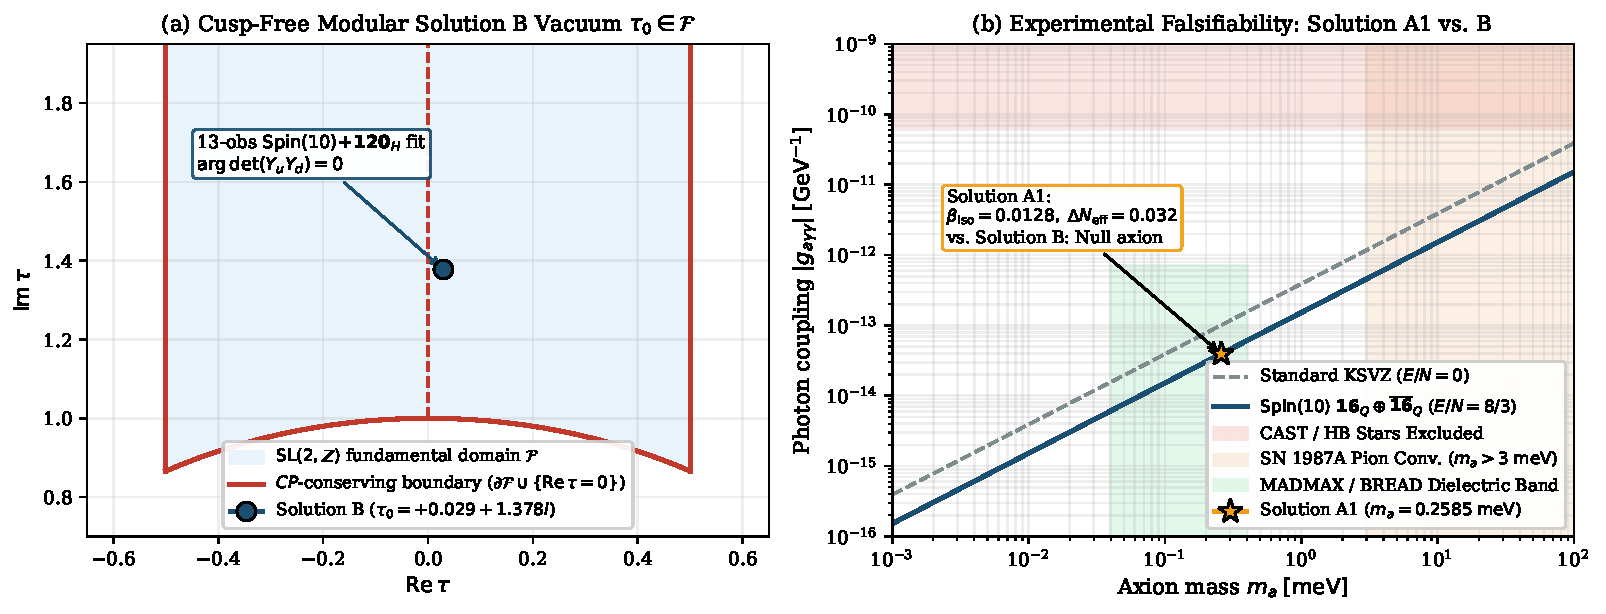
\includegraphics[width=0.98\textwidth]{../figures/fig3_modular_spin10_and_experimental_fork.pdf}
\caption{\textbf{(a)} Az $\mathrm{SL}(2,\mathbb{Z})$ fundamentális tartománya ($\mathcal{F}$) és a csúcspólus-mentes moduláris Solution B vákuuma ($\tau_0 = +0.02934 + 1.37758i \in \mathcal{F}$). \textbf{(b)} Kísérleti falszifikálhatósági térkép az $(m_a, |g_{a\gamma\gamma}|)$ síkon.}
\label{fig:hu-mod}
\end{figure}

Az axion elhagyása $M_R$ felett csúcspólus-mentes moduláris $\mathcal{N}=1$ szupergravitációt követel meg \cite{Feruglio2019Modular,KaplunovskyLouis1995,ChenRamosSanchezRatz2020,FeruglioStrumiaTitov2023}: a $K_{\mathrm{std}} = -3 M_{\mathrm{Pl}}^2\ln(-i(\tau-\bar{\tau}))$ potenciál ($W$ súlya $-3$), $k_{16} = (+6,0,-6)$, $k_H = +3$ ($\mathbf{10}_H,\overline{\mathbf{126}}_H,\mathbf{120}_H$) és Green--Schwarz $S$ dilaton mellett a nem-minimális Kähler-metrika \cite{ChenRamosSanchezRatz2020} $H = Z_{16}(\tau_0,\bar{\tau}_0)^{-1/2} > 0$ kanonizálója megőrzi az $\arg\det(Y_u Y_d) = 0$ feltételt. Egzisztenciabizonyításként (26 valós paraméter 13 kéthurkos egy-Higgs SM-sivatag megfigyelhetőre $M_R$-nél) szigorúan $\mathcal{F}$ belsejében ($\tau_0 = +0.02934 + 1.37758i$, $|\tau_0| = 1.3779 \ge 1.01$, \ref{fig:hu-mod}a.\ ábra) mind a 13 töltöttfermion- és CKM-megfigyelhető $\mathrm{loss} = 1.78\times 10^{-20}$ pontossággal illeszkedik ($\arg\det(Y_u Y_d) = -9.33\times 10^{-14}\;\mathrm{rad}$, $|\varepsilon_1| = 4.18\times 10^{-6}$), \textbf{de négy egyidejű UV-feltételt igényel}: (i) $M_{\mathrm{SUSY}} \ge M_R \gg T_{\max}$ (stabil LSP túlnyomás ellen), (ii) nem-holomorf Kähler-stabilizációt $\partial_\tau K(\tau_0,\bar{\tau}_0)=0$ valós $\tau$-független $W_{\mathrm{hidden}}(X)\in\mathbb{R}$ mellett, (iii) egyetlen SM Higgs-dublettet $M_R$ alatt ($y_b(M_R)/y_\tau(M_R) = 0.6173$, $\Delta\bar{\theta}_{\mathrm{SM}} \sim 10^{-16}$ \cite{EllisGaillard1979}, a $-4.87\times 10^{-3}\;\mathrm{rad}$ 2HDM-hurok elkerülésére), és (iv) a $\mathbf{120}_H$ multiplettet. Ez éles kísérleti elágazást ad (\ref{tab:hu-comp}.\ táblázat, \ref{fig:hu-mod}b.\ ábra) a MADMAX/BREAD \cite{Caldwell2017MADMAX,Liu2022BREAD}, LiteBIRD és CMB-S4 mérések számára.

\begin{table}[t!]
\centering
\caption{A tisztán 4D szuperszimmetria-mentes főmodell (\textbf{Solution A1}) és a moduláris $\mathcal{N}=1$ szupergravitációs alternatíva (\textbf{Solution B}) összehasonlítása.}
\label{tab:hu-comp}
\vspace{0.35em}
\renewcommand{\arraystretch}{1.18}
\begin{tabularx}{\textwidth}{>{\bfseries}l >{\raggedright\arraybackslash}X >{\raggedright\arraybackslash}X}
\toprule
Tulajdonság / Megfigyelhető & \textbf{Solution A1 ($\mathbb{Z}_{16}$ konformális axion)} & \textbf{Solution B (Moduláris $\mathrm{Spin}(10)\oplus\mathbf{120}_H$)} \\
\midrule
Téridő és SUSY-igény & Tiszta 4D nem-SUSY QFT (0 szuperpartner) & $\mathcal{N}=1$ SUGRA ($M_{\mathrm{SUSY}} \ge M_R$) \\
Mérték- / topológiai védelem & $\mathbb{Z}_{16}$ ($\Omega_5^{\mathrm{Spin}}(B\mathbb{Z}_{16}) \equiv 0$; 4D $\mathrm{U}(1)_g$ UV) & $\mathrm{SL}(2,\mathbb{Z})\rtimes CP$ + GS $S$ + $\partial_\tau K(\tau_0)=0$ \\
UV skalár / Kähler-feltevések & Technikailag természetes flaton-eltolás ($\lambda_\chi, c_{6,8} \ll 1$) & 26 paraméteres nem-minimális $Z_{16}$ + 4 UV-feltétel \\
Jósolt $|\bar{\theta}_{\mathrm{QCD}}|$ & $3.07\times 10^{-34}$ ($d = 16$) & $\sim 10^{-16}$ (4-hurkos egy-Higgs SM) \\
\cite{Olcsak2026Paper25} $G_{\mathrm{PS}}$ torony érintetlen? & \textbf{Igen} ($y_b(M_R)/y_\tau(M_R) = 0.6931$) & \textbf{Nem} (bidublettek lecsatolása $M_R$-nél $+ \mathbf{120}_H$) \\
\cite{Olcsak2026Paper24} $\eta_B$ és $n_s$ érintetlen? & \textbf{Igen} ($\delta\eta_B/\eta_B = -0.014\%$, $n_s = 0.9620$) & \textbf{Igen} ($M_{\mathrm{SUSY}} \ge M_R > T_{\max}$, $\varepsilon_1 \neq 0$) \\
Relikvia-sűrűség & $\Omega_a h^2 = 0.00159$ ($\theta_i=1$); $\Omega_\chi h^2 \equiv 0$ & $\Omega_{\mathrm{LSP}}h^2 \equiv 0 \iff M_{\mathrm{SUSY}} \gg T_{\max}$ \\
Dielektromos halószkóp jel & $m_a = 0.2585\;\mathrm{meV}$ (MADMAX / BREAD) & Szigorúan zérus minden $m_a$-ra \\
CMB izokurvatúra és $\Delta N_{\mathrm{eff}}$ & $\beta_{\mathrm{iso}} = 0.0128$ (LiteBIRD); $\Delta N_{\mathrm{eff}} = 0.032$ & $\beta_{\mathrm{iso}} \equiv 0$; $\Delta N_{\mathrm{eff}} \equiv 0$ \\
\bottomrule
\end{tabularx}
\end{table}

\subsection*{Reprodukálhatóság és kódelérhetőség}
Minden szimbolikus (\texttt{SymPy}), kéthurkos RGE, Boltzmann-, 75\,000 lépéses ODE- és 13-megfigyelhetős moduláris számítást önállóan reprodukál a \texttt{scripts/verify\_paper26\_strong\_cp\_closure.py} és a \texttt{scripts/generate\_paper26\_figures.py}.

\begin{thebibliography}{99}
\small
\raggedright
\setlength{\itemsep}{2pt}
\bibitem{Abel2020nEDM} C.~Abel \textit{et al.}, \emph{Phys.\ Rev.\ Lett.} \textbf{124}, 081803 (2020).
\bibitem{PDG2024} S.~Navas \textit{et al.} (Particle Data Group), \emph{Phys.\ Rev.\ D} \textbf{110}, 030001 (2024).
\bibitem{tHooft1976} G.~'t~Hooft, \emph{Phys.\ Rev.\ Lett.} \textbf{37}, 8 (1976).
\bibitem{JackiwRebbi1976} R.~Jackiw és C.~Rebbi, \emph{Phys.\ Rev.\ Lett.} \textbf{37}, 172 (1976).
\bibitem{CallanDashenGross1976} C.~G.~Callan, R.~F.~Dashen és D.~J.~Gross, \emph{Phys.\ Lett.\ B} \textbf{63}, 334 (1976).
\bibitem{PospelovRitz2005} M.~Pospelov és A.~Ritz, \emph{Annals Phys.} \textbf{318}, 119 (2005).
\bibitem{PecceiQuinn1977} R.~D.~Peccei és H.~R.~Quinn, \emph{Phys.\ Rev.\ Lett.} \textbf{38}, 1440 (1977).
\bibitem{Weinberg1978} S.~Weinberg, \emph{Phys.\ Rev.\ Lett.} \textbf{40}, 223 (1978).
\bibitem{Wilczek1978} F.~Wilczek, \emph{Phys.\ Rev.\ Lett.} \textbf{40}, 279 (1978).
\bibitem{Kim1979} J.~E.~Kim, \emph{Phys.\ Rev.\ Lett.} \textbf{43}, 103 (1979).
\bibitem{ShifmanVainshteinZakharov1980} M.~A.~Shifman, A.~I.~Vainshtein és V.~I.~Zakharov, \emph{Nucl.\ Phys.\ B} \textbf{166}, 493 (1980).
\bibitem{Zhitnitsky1980} A.~R.~Zhitnitsky, \emph{Sov.\ J.\ Nucl.\ Phys.} \textbf{31}, 260 (1980).
\bibitem{DineFischlerSrednicki1981} M.~Dine, W.~Fischler és M.~Srednicki, \emph{Phys.\ Lett.\ B} \textbf{104}, 199 (1981).
\bibitem{KamionkowskiMarchRussell1992} M.~Kamionkowski és J.~March-Russell, \emph{Phys.\ Lett.\ B} \textbf{282}, 137 (1992).
\bibitem{Holman1992} R.~Holman \textit{et al.}, \emph{Phys.\ Lett.\ B} \textbf{282}, 132 (1992).
\bibitem{BarrSeckel1992} S.~M.~Barr és D.~Seckel, \emph{Phys.\ Rev.\ D} \textbf{46}, 539 (1992).
\bibitem{DiLuzio2020} L.~Di~Luzio, M.~Giannotti, E.~Nardi és L.~Visinelli, \emph{Phys.\ Rept.} \textbf{870}, 1 (2020).
\bibitem{Nelson1984} A.~E.~Nelson, \emph{Phys.\ Lett.\ B} \textbf{136}, 387 (1984).
\bibitem{Barr1984} S.~M.~Barr, \emph{Phys.\ Rev.\ Lett.} \textbf{53}, 329 (1984).
\bibitem{BabuMohapatra1990} K.~S.~Babu és R.~N.~Mohapatra, \emph{Phys.\ Rev.\ D} \textbf{41}, 1286 (1990).
\bibitem{Kuchimanchi1996} R.~Kuchimanchi, \emph{Phys.\ Rev.\ Lett.} \textbf{76}, 3486 (1996).
\bibitem{DineKramerNir1997} M.~Dine, R.~G.~Leigh és A.~Kagan, \emph{Phys.\ Rev.\ D} \textbf{48}, 2214 (1993); M.~Dine és P.~Draper, \emph{JHEP} \textbf{08}, 132 (2015).
\bibitem{HallHarigaya2018} L.~J.~Hall és K.~Harigaya, \emph{JHEP} \textbf{10}, 130 (2018).
\bibitem{ValentiVecchi2021} A.~Valenti és L.~Vecchi, \emph{JHEP} \textbf{07}, 203 (2021).
\bibitem{FeruglioStrumiaTitov2023} F.~Feruglio, A.~Strumia és A.~Titov, \emph{JHEP} \textbf{07}, 027 (2023).
\bibitem{Olcsak2026Zenodo} J.~Olcsak, Zenodo (2026), \href{https://doi.org/10.5281/zenodo.19120268}{doi:10.5281/zenodo.19120268}.
\bibitem{Olcsak2026Paper23} J.~Olcsak, Zenodo v12.2.0 (2026), \href{https://doi.org/10.5281/zenodo.24372826}{doi:10.5281/zenodo.24372826}.
\bibitem{Olcsak2026Paper24} J.~Olcsak, Zenodo v1.1.0 (2026), \href{https://doi.org/10.5281/zenodo.24380371}{doi:10.5281/zenodo.24380371}.
\bibitem{Olcsak2026Paper25} J.~Olcsak, Zenodo v1.1.0 (2026), \href{https://doi.org/10.5281/zenodo.24392639}{doi:10.5281/zenodo.24392639}.
\bibitem{Starobinsky1980} A.~A.~Starobinsky, \emph{Phys.\ Lett.\ B} \textbf{91}, 99 (1980).
\bibitem{Whitt1984} B.~Whitt, \emph{Phys.\ Lett.\ B} \textbf{145}, 176 (1984).
\bibitem{Milgrom2010QUMOND} M.~Milgrom, \emph{Mon.\ Not.\ Roy.\ Astron.\ Soc.} \textbf{403}, 886 (2010).
\bibitem{Planck2018Inflation} Y.~Akrami \textit{et al.} (Planck Collaboration), \emph{Astron.\ Astrophys.} \textbf{641}, A10 (2020).
\bibitem{Planck2018Cosmo} N.~Aghanim \textit{et al.} (Planck Collaboration), \emph{Astron.\ Astrophys.} \textbf{641}, A6 (2020).
\bibitem{IbanezRoss1991} L.~E.~Ibáñez és G.~G.~Ross, \emph{Phys.\ Lett.\ B} \textbf{260}, 291 (1991).
\bibitem{Hsieh2018} C.-T.~Hsieh, \href{https://arxiv.org/abs/1808.02881}{arXiv:1808.02881 [hep-th]} (2018).
\bibitem{GarciaEtxebarriaMontero2019} I.~García-Etxebarria és M.~Montero, \emph{JHEP} \textbf{08}, 003 (2019).
\bibitem{BarrChangSenjanovic1991} S.~M.~Barr, D.~Chang és G.~Senjanović, \emph{Phys.\ Rev.\ Lett.} \textbf{67}, 2765 (1991).
\bibitem{BentoBrancoParada1991} L.~Bento, G.~C.~Branco és P.~A.~Parada, \emph{Phys.\ Lett.\ B} \textbf{267}, 95 (1991).
\bibitem{AntuschSpinrath2011} S.~Antusch, M.~Holthausen, M.~A.~Schmidt és M.~Spinrath, \emph{Nucl.\ Phys.\ B} \textbf{877}, 752 (2013).
\bibitem{Carenza2021SN} P.~Carenza \textit{et al.}, \emph{Phys.\ Rev.\ Lett.} \textbf{126}, 071102 (2021).
\bibitem{Lella2024SN} A.~Lella \textit{et al.}, \emph{Phys.\ Rev.\ D} \textbf{109}, 023001 (2024).
\bibitem{Buschmann2022NS} M.~Buschmann \textit{et al.}, \emph{Phys.\ Rev.\ Lett.} \textbf{128}, 091102 (2022).
\bibitem{MachacekVaughn1984} M.~E.~Machacek és M.~T.~Vaughn, \emph{Nucl.\ Phys.\ B} \textbf{236}, 221 (1984).
\bibitem{LuoXiao2003} M.-x.~Luo és Y.~Xiao, \emph{Phys.\ Rev.\ Lett.} \textbf{90}, 011601 (2003).
\bibitem{Buttazzo2013} D.~Buttazzo \textit{et al.}, \emph{JHEP} \textbf{12}, 089 (2013).
\bibitem{SalvioStrumiaWetterich2014} A.~Salvio, A.~Strumia és W.~Xue, \emph{JCAP} \textbf{01}, 011 (2014).
\bibitem{NotariRompineveVilladoro2023} A.~Notari, F.~Rompineve és G.~Villadoro, \emph{Phys.\ Rev.\ Lett.} \textbf{131}, 011004 (2023).
\bibitem{Linde1991Axion} A.~D.~Linde, \emph{Phys.\ Lett.\ B} \textbf{259}, 38 (1991).
\bibitem{HarigayaIbeKawasakiYanagida2015} K.~Harigaya, M.~Ibe, M.~Kawasaki és T.~T.~Yanagida, \emph{JCAP} \textbf{11}, 003 (2015).
\bibitem{KasuyaKawasakiYanagida1997} S.~Kasuya, M.~Kawasaki és T.~Yanagida, \emph{Phys.\ Lett.\ B} \textbf{409}, 94 (1997).
\bibitem{Randall1992} L.~Randall, \emph{Phys.\ Lett.\ B} \textbf{284}, 77 (1992).
\bibitem{RediSato2016} M.~Redi és R.~Sato, \emph{JHEP} \textbf{05}, 104 (2016).
\bibitem{ContinoPodoRevello2022} R.~Contino, A.~Podo és F.~Revello, \emph{JHEP} \textbf{04}, 180 (2022).
\bibitem{Feruglio2019Modular} F.~Feruglio, in \emph{From My Vast Repertoire\dots: Guido Altarelli's Legacy}, World Scientific, pp.~227--266 (2019).
\bibitem{KaplunovskyLouis1995} V.~Kaplunovsky és J.~Louis, \emph{Nucl.\ Phys.\ B} \textbf{444}, 191 (1995).
\bibitem{ChenRamosSanchezRatz2020} M.-C.~Chen, S.~Ramos-Sánchez és M.~Ratz, \emph{Phys.\ Lett.\ B} \textbf{801}, 135153 (2020).
\bibitem{EllisGaillard1979} J.~R.~Ellis és M.~K.~Gaillard, \emph{Nucl.\ Phys.\ B} \textbf{150}, 141 (1979).
\bibitem{Caldwell2017MADMAX} A.~Caldwell \textit{et al.} (MADMAX Working Group), \emph{Phys.\ Rev.\ Lett.} \textbf{118}, 091801 (2017).
\bibitem{Liu2022BREAD} J.~Liu \textit{et al.} (BREAD Collaboration), \emph{Phys.\ Rev.\ Lett.} \textbf{128}, 131801 (2022).
\end{thebibliography}

\end{document}
